%%%%%%%%%%%%%%%%%%%%%%%%%%%%%%%%%%%%%%%%%
% Lab Book 
% Original author:
% Frank Kuster (http://www.ctan.org/tex-archive/macros/latex/contrib/labbook/)
%
% Important note:
% This template requires the labbook.cls file to be in the same directory as the
% .tex file. The labbook.cls file provides the necessary structure to create the
% lab book.
%
%
% HOW TO USE THIS TEMPLATE 
% Each day in the lab consists of three main things:
%
% 1. LABDAY: The first thing to put is the \labday{} command with a date in 
% curly brackets, this will make a new page and put the date in big letters 
% at the top.
%
%%%%%%%%%%%%%%%%%%%%%%%%%%%%%%%%%%%%%%%%%

%----------------------------------------------------------------------------------------
%	PACKAGES AND OTHER DOCUMENT CONFIGURATIONS
%----------------------------------------------------------------------------------------

\documentclass[idxtotoc,hyperref,openany]{labbook} % 'openany' here removes the gap page between days, erase it to restore this gap; 'oneside' can also be added to remove the shift that odd pages have to the right for easier reading

\usepackage[ 
  backref=page,
  pdfpagelabels=true,
  plainpages=false,
  colorlinks=true,
  bookmarks=true,
  pdfview=FitB]{hyperref} % Required for the hyperlinks within the PDF
  
\usepackage{booktabs} % Required for the top and bottom rules in the table
\usepackage{float} % Required for specifying the exact location of a figure or table
\usepackage{graphicx} % Required for including images
\usepackage[parfill]{parskip}
\usepackage{amsmath}
\usepackage{amssymb}
\graphicspath{{./images/}}

\newlength{\mylen}
\setbox1=\hbox{$\bullet$}\setbox2=\hbox{\tiny$\bullet$}
\setlength{\mylen}{\dimexpr0.5\ht1-0.5\ht2}
\renewcommand\labelitemi{\raisebox{\mylen}{\tiny$\bullet$}}

\newcommand{\HRule}{\rule{\linewidth}{0.5mm}} % Command to make the lines in the title page
\setlength\parindent{0pt} % Removes all indentation from paragraphs

%----------------------------------------------------------------------------------------
%	DEFINITION OF EXPERIMENTS
%----------------------------------------------------------------------------------------

%\newexperiment{shorthand}{Description of the experiment}

%---------------------------------------------------------------------------------------

\begin{document}

%----------------------------------------------------------------------------------------
%	TITLE PAGE
%----------------------------------------------------------------------------------------

\frontmatter % Use Roman numerals for page numbers
\title{
\begin{center}
\HRule \\[0.4cm]
{\Huge \bfseries Research Journal}\\
\HRule \\[1.5cm]
\end{center}
}
\author{\Huge Jerome Wynne \\ \\ \LARGE University of Bristol \\[2cm]}
\date{19th June 2017 - Present}
\maketitle

\tableofcontents

\mainmatter

%----------------------------------------------------------------------------------------
%	LAB BOOK CONTENTS
%----------------------------------------------------------------------------------------

% Blank template to use for new days:

%\labday{Day, Date Month Year}

%\experiment{}

%Text

%-----------------------------------------

%\experiment{}

%Text

%----------------------------------------------------------------------------------------

\labday{Thursday, 1st June 2017}
\experiment{Summary}
\begin{itemize}
	\item Set up this labbook.
	\item Wrote down what I'd like to achieve during my placement.
	\item Listed a bunch of classic \emph{Computer Vision} papers.
\end{itemize}

\experiment{Placement objectives}
During my 8-week placement I would like to:
\begin{itemize}
	\item Apply and understand the most useful \emph{Computer Vision} algorithms.
	\item Write either a statistics, machine learning, or \emph{Computer Vision} research paper worthy of publication.
	\item Develop a systematic workflow to problems involving data, and demonstrate this workflow in publicly available scripts or notebooks.
\end{itemize}

\experiment{Reading a paper critically}
\begin{itemize}
\item Motivations for the problem posed
\item The choices made in finding a solution
\item The assumptions behind the solution
\item The validity of those assumptions
\item Whether assumptions can be removed without invalidating the approach
\item What was accomplished
\item Future research directions
\end{itemize}
\newpage

\experiment{Structuring your time}
I think it's realistic to aim for 12 hours of productive work each day. This includes reading, studying, and running my own experiments. To begin with, I think I should spend at least three-quarters of this time learning. Maybe by week four I will shift the ratio.

 I will see how it goes, but I suspect I will prefer to work from the University rather than DNV-GL's offices.
 
 To make this placement a success, I will need to be disciplined about how I use my time. I know that if I get up early and immediately go to work, I can easily crack out four hours without breaking a sweat. After this time I can take at least a couple of hours - go to the gym, read, walk, or - of course - eat. After that I'll get back on that horse for another four or five hours, before taking another short break, then do a few more hours.
 
 Having lots of sleep is important for my mental health and emotional wellbeing, so I should aim to get at least eight hours. If I get up at six, this means that I should go to bed at half-nine. I can work from my flat, University buildings, or the DNV-GL offices. It would be a good idea to mix the places I study up - I know this has helped me keep focused in the past. I need to be careful to provide some time for myself too, so that I can recuperate: I think two hours at the end of the day, eight until ten, will be enough.
 
 \experiment{Figuring out what to write about}
 \begin{enumerate}
 \item Narrow down your field of study
 \item Define what to investigate
 \item Establish a thesis or an argument
 \end{enumerate}

I am studying \emph{Computer Vision} and statistics. This is because I want to build robust algorithms to understand visual information, which in turns makes it easier to automate difficult or tedious tasks, such as watching CCTV cameras or spotting damage to structures in video footage. I am doing this so that we will know more about how patterns in visual information can be found, and so that we can exploit these patterns to automate economically and socially beneficial tasks. I am also interested in how we can represent visual information to make it easier to work with and to understand.

\experiment{Structuring your work}
\begin{enumerate}
\item Find data that poses an unsolved problem, or find a problem that needs data to be solved.
\item Find the data, or pose the problem.
\item Review the relevant literature.
\item Propose a solution, then run experiments and conduct analysis to test that solution.
\item Write up the results.
\end{enumerate}

\experiment{How to use this book}
I should use this book to record what I'm doing, ideas and conversations I have, experiments I run, papers and books to read, things I understand and don't understand - everything related to my research. It only takes a few minutes to put a screenshot in this document - remember this!

As a habit, at the beginning of each day I will write down what I plan to do. At the end of the day I'll review what I've done. I should also review the book each week, to get an idea what I've been up to and where I'm headed.

\newpage
%-----------------------------------------------
 % 		PAPERS
 %---------------------------------------------
{\hspace{5cm} \Huge\textbf{Papers} \hfill}
\\

\begin{table}[h!]
\hspace{-2.5cm}
\centering
\renewcommand{\arraystretch}{1.5}
 \small
\begin{tabular}{@{}p{6cm} p{4cm} p{1cm} p{3cm} p{1cm}} \toprule
\textbf{Title}		&	\textbf{Authors}	&	\textbf{Year}		&	\textbf{Topic}		& 	\textbf{Read}\\ \midrule
Theory of Edge Detection	&	D. Marr, E. Hildreth	&	1980	&	Computer vision	& No \\
A Computational Approach to Edge Detection & J. Canny & 1986 & \emph{Computer Vision} & No \\
Determining optical flow	&	B.K.P. Horn, B. Schunk	&	1981	&	Computer vision	&	No \\
An iterative image registration technique with an application to stereo vision	&	B. Lucas, T. Kanade	& 1981 &	Computer vision	&	No \\
Snakes: Active contour models	&	M. Kass, A. Witkin, D. Terzpoulos	&	1988 & \emph{Computer Vision} & No \\
Eigenfaces for recognition & M. Turk, A. Pentland & 1991 & \emph{Computer Vision} & No \\
Shape and motion from image streams under orthography: a factorization method & C. Tomasi, T. Kanade & 1992 & \emph{Computer Vision} & No \\
Texture features for browsing and retrieval of image data & B. Manjunath, W. Ma & 1996 & \emph{Computer Vision} & No\\
Conditional density propagation for visual tracking & M. Isard, A. Blake & 1998 & \emph{Computer Vision} & No \\
Normalized cuts & J. Shi, J. Malik & 2000 & \emph{Computer Vision} & No \\
Non-parametric model for background subtraction & A. Elgammal, D. Harwood, L. Davis & 2000 & \emph{Computer Vision} & No\\
Distinctive image features from scale-invariant keypoints & D. Lowe & 2004 & \emph{Computer Vision} & No
 \\ \bottomrule
\end{tabular}
\end{table}


\labday{Monday, 19th June 2017}
\experiment{Summary}
\begin{itemize}
\item Arrived at DNV offices @ 10:00.
\item H \& S induction. Remember to look at the green lights above the doors!
\item Met Elizabeth Traiger:
\begin{itemize}
\item Solar panel cracks toy problem.
\item DNV are keen to use Python.
\item Approx. 1500 minutes of turbine data available.
\item We need a method for labeling the data.
\end{itemize} 
\item IT was not set up - she will email me tomorrow when it is ready.
\item DNV use Microsoft Azure services internally.
\item The company is open to using TensorFlow.
\item We agreed that weekly meetings would be appropriate. She is away this Friday (in London, speaking about using satellite imagery of windfarms to monitor fish populations (?), in association with the European Space Agency) and next week (site visit?).
\item Various ideas came up in our conversation: super-resolution methods, using simulation data, creating synthetic data, thinking about how to segment the images.
\item Footage from two turbines is available this week. More footage will be available next week.
\item I can VPN into DNV's network using the laptop that they provided me.
\item I left the DNV offices after lunch (14:00), then worked on the Design Project briefs until 16:30.
\item Liz planned to book a meeting with the inspections team to discuss how they look for damage. Possible questions:
\begin{itemize}
	\item What does damage look like?
	\item Over what time periods does it develop?
	\item What causes the damage?
	\item What mistakes do you make when looking for damage?
	\item What type of damage is easiest/most difficult to spot?
	\item What do you do when you find damage?
	\item What problems do you think there are with using drones to identify damage?
\end{itemize}
\end{itemize}

In the afternoon I read the introduction to Canny's paper on edge detection. I learnt that there is a tension between edge detection and localization (the distance between the detected edge and the true edge). Apparently the paper determines the optimal operator for various common edges.

I also read the introduction and first chapter of S.J. Prince's book on computer vision. The introduction outlined the book's structure and the first chapter was a quick review of basic probability theory.

\begin{itemize}
\item Read Canny paper.
\item Read the Chapter 1, 3, and 6 of S.J. Computer Vision. Make notes and complete the associated exercises.
\item Apply what was learnt in this chapter using Python.
\item Outline the structure of compute vision / machine learning.
\end{itemize}

\experiment{Prince: \emph{Computer Vision} (Ch. 1, Introduction)}
The book's structure was outlined. It consists of six sections:
\begin{enumerate}
\item Probability.
\item Machine learning for machine vision.
\item Graphical models (principled ways to simplify the relationship between image data and estimated properties) for machine vision.
\item Image preprocessing.
\item Geometric machine vision - generating 3D models based on image data and localizing a camera based on its view.
\item Families of machine vision models for common problems.
\end{enumerate}
It took me about ten minutes to read through this first chapter of five pages. Relevant papers are listed at the end of each of the book's sections.

\experiment{Prince: \emph{Computer Vision} (Ch. 2, Introduction to Probability)}
The second chapter took about an hour to read and make notes for. Almost all of it was review material: random variables, distributions, joint distributions, Bayes' rule, conditionality, and expectation. I did learn, however, two useful things:
\begin{itemize}
\item A Hinton diagram can be used to visualize probability mass functions. A square is associated with each point; the square's area relative to the total area of all squares corresponds to that value's relative probability. Figure \ref{fig:hinton_diagram} shows a Hinton diagram in two variables.
\begin{figure}[h!]
\centering
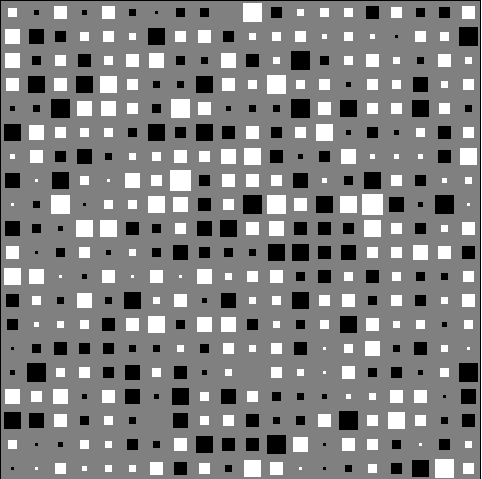
\includegraphics[width=0.5\textwidth]{hinton_diagram.png}
\caption{A Hinton diagram can be used to visualize probability mass functions in one or two variables.}
\label{fig:hinton_diagram}
\end{figure}
\item A useful identity: if two random variables are independent, then the product of their expectation is equivalent to the expectation of their product. More generally:
\begin{equation}
	E[f(x) \cdot g(y)] = E[f(x)] \cdot E[g(y)]
\end{equation}
\end{itemize}



\labday{Tuesday, 20th June 2017}
\experiment{Summary}
I woke at six (I'm getting the hang of it). For the first hour of the day I reviewed the project brief MZ had commented on and sent it off to PH. PH mentioned I could use his office for the next two weeks while he was away - hopefully I can pick up the key from him this afternoon.

Today I would like to complete Chapters 3 and 4 of Prince's Computer Vision, do some modeling in Python, and begin the CVX course. I should also get an overview of the main \emph{Computer Vision} tools for Python.

I made notes on Chapter 3 and completed five of its exercises, which related to conjugacy, the exponential family, and the modes of the distributions studied. PH said to pick up the key to his office from the porter. ET emailed me to say that IT have set up my account - I agreed to go in tomorrow morning to meet her and pick up my laptop. I should also ask her when we plan to meet the wind turbine inspections team.

I intend to complete Chapter 4 this afternoon. I am now going to read Canny's paper.
I tried to read Canny's paper but kept zoning out. I did understand, however, that he formulated an optimization problem by expressing detection performance as signal-to-noise ratio and localization performance as a similar quantity but involving gradients.

I spent fifty minutes reading through Chapter 4. I made notes on maximum likelihood, maximum a posteriori, and bayesian methods for optimizing parameter estimates. I read through an example wherein the mean and variance of a univariate normal distribution were estimated using a normal-scaled inverse gamma prior; as it turns out, the benefits of using the conjugate here are twofold - not only does the posterior have a closed-form solution, but so also does the posterior predictive!

\experiment{Prince: \emph{Computer Vision} (Ch. 3, Common Probability Distributions)}

I started on Chapter 3 of Prince's book yesterday. It covers eight probability distributions that will be useful for machine vision purposes. Four of these are for modelling image data or world properties; the other four are for modelling the parameters of these four. I made notes, but have yet to complete the exercises. The distribution pairs covered were:
\begin{itemize}
	\item Bernoulli - Beta
	\item Categorical - Dirichlet
	\item Univariate normal - Normal-scaled inverse gamma
	\item Multivariate normal - Normal inverse Wishart
\end{itemize}
The four distributions on the left were familiar to me, as was the beta distribution (however it was useful to note that the expectation of $\text{Beta}[\alpha, \beta]$ is defined by $\frac{\alpha}{\alpha + \beta}$). The Dirichlet, normal-inverse scaled gamma, and normal inverse wishart distributions were new to me. 

The Dirichlet distribution is effectively a generalization of the beta distribution to cover more than one variable. It's used to model the $K$ parameters of a categorical distribution. As such, $\sum_k \lambda_k = 1$ at all points in the Dirichlet distribution. Its hyperparameters $\alpha_1, ..., \alpha_K$ describe the categorical distribution's expecations over each of its variables $E[\lambda_1], ..., E[\lambda_K]$; the magnitude of the $\alpha$ values determines the Dirichlet's dispersion.

The Normal-scaled inverse gamma distribution is used to model uncertainty in the mean and variance of a univariate normal distribution. It has four parameters. In a similar vein, the normal inverse Wishart distribution describes uncertainty in the mean vector and covariance matrix of a multivariate normal distribution.

I'm now going to complete three questions from the exercises, then go to the barbers. When I get back I will complete three more exercises, before continuing to read the Canny paper.

I completed three questions. The first asked for the mode of the beta distribution (found by maximizing the pdf w.r.t. the variable). The second pointed out that all of the distributions in the chapter were members of the exponential family; it then requested the beta pdf in exponential family form. The third related a normal prior and restricted normal likelihood to a normal posterior (i.e. it was a conjugacy problem). These questions together took me about forty-five minutes to complete.

This is not the first time the exponential distribution has been mentioned - why is understanding multiple distributions as variants on one distribution useful?

I completed two more questions: showing that the normal-scaled inverse gamma is the conjugate prior to the univariate normal distribution; showing that the Dirichlet distribution is the conjugate prior to the categorical distribution. They were mostly exercises in algebra, but it did drive home why the Dirichlet and normal-scaled inverse gamma distributions are relevant, and what they look like (particularly w.r.t. the Dirichlet-beta similarities).

\experiment{Prince: \emph{Computer Vision} (Ch. 4, Fitting Probability Models)}
The chapter began with maximum likelihood, maximum a posteriori, and bayesian methods for optimizing parameter estimates. I read through an example in which the mean and variance of a univariate normal distribution were estimated using a normal-scaled inverse gamma prior; as it turns out, the benefits of using the conjugate here are twofold - not only does the posterior have a closed-form solution, but so also does the posterior predictive! I think I would benefit from writing out the Bayesian solution, and possibly running a simulation in Python. Maybe I'll go through the other example before building the simulation.

I made notes on both worked examples. The second example involved inferring posterior and posterior predictive distributions from a categorical likelihood and its conjugate (a Dirichlet prior). As in the case of the univariate normal - normal-scaled inverse gamma problem, bott distributions had neat solutions. The posterior was another Dirichlet distribution (with correspondingly updated parameters $\tilde{\alpha}_j = \alpha_j + N_j$) and the posterior predictive turned out to be a function of beta functions.

I'm going to write two R simulations, one for each example.

I built an R simulation for the first example.

I attempted Q4.6, but fell short (the algebra became untangled). I will try again tomorrow morning; perhaps doing Q4.5 first will make it slightly easier. Once I've done those two questions, I should like to do Q4.7-4.10.
Worked 4 - 7:30 on Com. Vis. Chapter 4.

This evening I watched the first lecture from the CVX course. It explained what convex optimisation is, common variants of it (least squares and linear programming), discussed application areas, defined a convex functoin, provided an overview of the course, and gave some history on the topic.




\labday{Wednesday, 21st June 2017}
\experiment{Summary}
Today I plan to:
\begin{itemize}
	\item Complete the exercises from Ch. 4 of Computer Vision
	\item Walk through one of the examples available at PyImageSearch
	\item Read Ch. 5 of \emph{Computer Vision} and complete the associated exercises
	\item Pick up Paul Harper's office key
	\item Meet ET at 10:00 to have IT induction
	\item Explore solar panel dataset
	\item Investigate Python tools for tagging images
	\item Read Chapter 1 of Boyd's Convex Optimisation
\end{itemize}

(07:00 - 09:50) 
I spent the first hour and forty-five minutes of the day completing Exercises 4.5 - 4.10 of Computer Vision. I then made notes on Chapter 5, which is focused on the normal distribution. It began by showing the difference between spherical, diagonal, and full covariance matrices - spherical matrices have circular isodensity contours, diagonals have ellipsoidal ones whose axes are aligned with coordinate axes, and full covariance matrices have ellipsoidal contours in any orientation.

As it happens, it's possible to rotate a distribution's coordinate system to permit a full covariance matrix to be reexpressed as a diagonal one. The rotation matrix is deduced using the singular value decomposition (something I should probably know, but don't). I'm about to head off to DNV, but I intend to watch Gilbert Strang's lecture on the singular value decomposition when I get back. I think I could also do with inspecting matrix inverses more closely.

I spent the afternoon (10:30 - 16:00) in the DNV offices getting set-up with IT and so on. I also went through the two datasets made available to me so far. In the evening I wrote a Python script to resize and subset the PV panel images. I also skimmed Ch. 6 of Computer Vision.

Tomorrow morning I should label a few hundred of these images and try out the algorithms described in Ch. 6 of Com. Vis. For the first three hours of the day I should like to study from the book. The middle hours can be spent labelling and coding, before returning again to studying. I will read through Ch. 1 of S. Boyd's book on convex optimization also.

I did find a tool for annotating images - it's called Fiji (https://fiji.sc/). I should really start time-stamping my entries on this...

I also read a paper [\emph{Detection and Classification of Surface Defects on Gun Barrels Using Computer Vision and Machine Learning}, Sanmuhamani et al.] on gun barrel damage classification. They had success using an extended maxima transform was used to segment their images. They used sequential forward-feature selection. The six features that presented themselves as most useful (in a texture-based classification problem, fed into a radial-basis SVM) were:
\begin{itemize}
	\item Mean
	\item Variance
	\item Smoothness
	\item Skewness
	\item Uniformity
	\item Entropy
\end{itemize}
I think it would be worthwhile getting the definitions for these should any texture-based classification work come up.

I need to start logging to-dos using the Office 365 Planner app.

\experiment{PV Panels}
The first dataset is a ~50 scans of PV panels. Possible objectives with these panels are:
\begin{itemize}
	\item Detecting cracks.
	\item Detecting pit marks.
	\item Detecting blown cells.
\end{itemize}
An example image is shown in Figure \ref{fig:example_pv_cell}. I made a repo for the PV project.

\begin{figure}
\centering
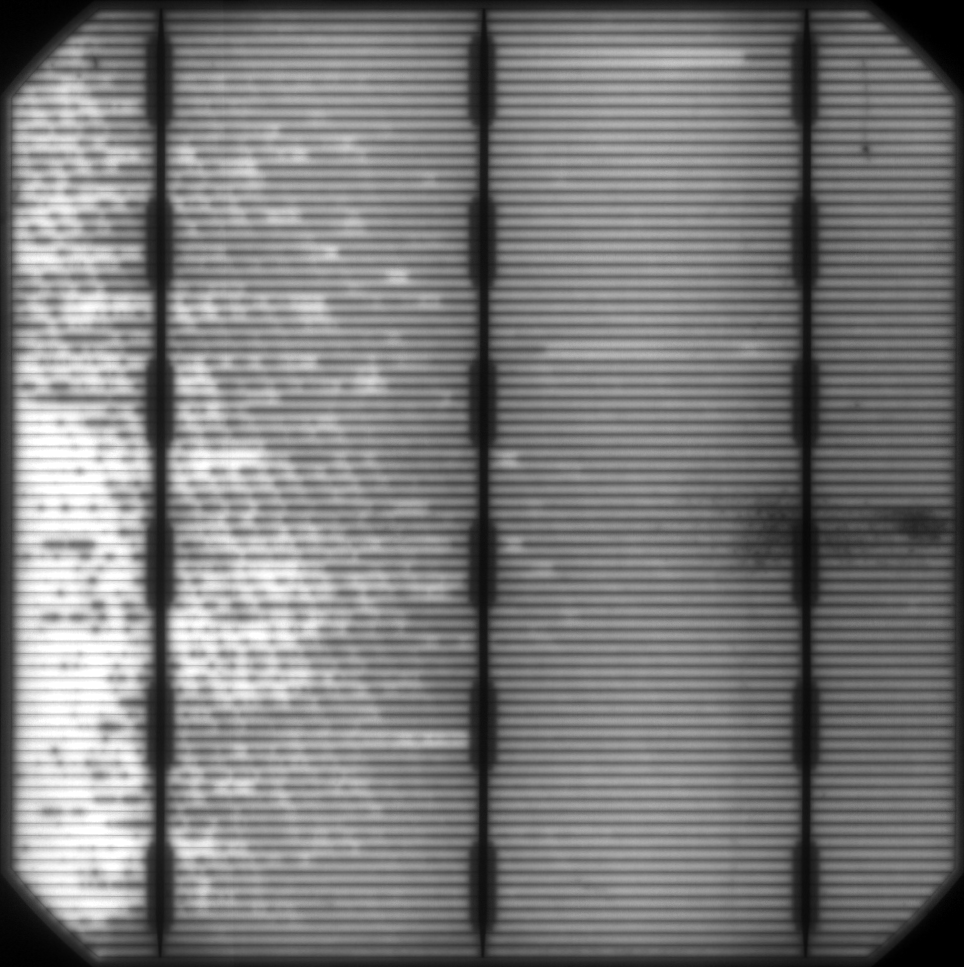
\includegraphics[width=0.5\textwidth]{pv_cell.png}
\caption{A sample image from the PV panels dataset.}
\label{fig:example_pv_cell}
\end{figure}

\experiment{PV Panels: Crack detection}
The objective of this task is to label images as according to whether or not they contain a crack - I don't think bounding boxes are appropriate. I'm going to begin by:
\begin{itemize}
	\item Rescaling the images to a constant size.
	\item Labeling the panels according to the damage they've incurred.
	\item Sorting the panels according to their type.
\end{itemize}

I created \texttt{panel-resizer.ipynb} to rescale the panel images to a fixed size\footnote{I deleted one duplicated image (52) and removed three smaller images}. This took me about an hour. While doing this, I realized that I could cluster the panels according to their metropolis distance from one another, generate an `undamaged' panel for each class, then use subtraction to identify damaged panels. I think the biggest weakness with such an approach, however, is the need for an `undamaged' panel image. How is easy would this be to generate synthetically?
\begin{enumerate}
	\item Label images (crack/no crack).
	\item 70/30 split of training/test data.
	\item Benchmark `dumb' classifiers.
	\item Select the best dumb classifier and optimize it.
\end{enumerate}


\labday{Thursday, 22nd June 2017}
\experiment{Summary}
Today I planned to:
\begin{itemize}
	\item Review what I covered yesterday.
	\item Read the blog post ``Classifying plankton with deep neural networks''.
	\item Label at least 50\% of the PV panel data.
	\item Set up a LaTeX report for the PV panel data.
	\item Update my current strategy for the PV data on Office 365.
	\item Complete problem exercises from Ch. 6 of \emph{Computer Vision}.
	\item Implement the algorithms presented in Ch. 6 of \emph{Computer Vision} on a dummy dataset.
	\item Benchmark 3 dumb classifiers against the labeled PV panel data.
	\item Read Ch. 1 of Boyd's \emph{Convex Optimisation}.
\end{itemize}
If there is time I will also begin reading Ch. 7 of \emph{Computer Vision}.

(07:30 - 08:00) I planned my approach to the PV panel crack detection task on Office 365.

(08:00 - 11:00) 

\experiment{PV Panels: Crack Detection}
To-dos:
\begin{itemize}
	\item Label subset images
	\item Build augmented images dataset
	\item Set up report
	\item Benchmark simple classifiers against augmented images
	\item Optimize best simple classifier
	\item Record simple classifier performances in report
	\item Set up Azure instance and train convnet against augmented images
	\item Upload augmented images dataset
	\item Investigate clustering of panels
\end{itemize}

\experiment{Prince: \emph{Computer Vision} (Ch. 5/6)}
Yesterday my work from this book constituted reviewing the many properties of the multivariate normal distribution, among which were:
\begin{itemize}
	\item The marginal distribution of a subset of a vector of normal r.v.s is also normal.
	\item The conditional distribution of a subset of vector of normal r.v.s, given the other r.v.'s values, is also a normal distribution.
	\item Its covariance matrix an be diagonalized using the singular value decomposition, which forms a rotation matrix that twists the reference frame to align with the axes of the distribution's ellipsoidal isodensity contours.
	\item It can have one of three types of covariance matrix - spherical, diagonal, or full - which determines how elliptical its isodensity contours are and what its orientation relative to the coordinate axes is.
\end{itemize}
In the evening I began work on Ch. 6, \emph{Learning and Inference in Vision}. It defined the basic task of machine vision as inferring world properties based on image data. It also outlined a framework for solving this problem consisting of three components:
\begin{itemize}
	\item A model relating image data to world properties.
	\item A learning algorithm for adjusting that model's parameters based on observations.
	\item An inference algorithm for returning a predicted world state based on input image data.
\end{itemize}
The model can be either discriminative or generative. A discriminative model describes $\text{Pr}(\mathbf{w}|\mathbf{x})$, the world state based on the image data. By contrast, a generative model instead represents the likelihood $\text{Pr}(\mathbf{x}|\mathbf{w}$) - what the image data should be for a given world state.

(08:20 - 9:20) Made notes on modeling a univariate continuous response with univariate continuous inputs using discriminative and generative methods. Also described how to model a binary response in terms of continuous image data, again via both generative and discriminative methods. 
 
\begin{itemize}
\item Univariate continuous data $x$, univariate continuous world state $w$
	\begin{itemize}
		\item Discriminative approach: Model $\text{Pr}(w|x)$ using $\text{Norm}_{w}[\phi_0 + \phi_1 x, \sigma^2]$. Fit $(\phi_0, \phi_1, \sigma^2)$ based on training set $\{x_i, w_i\}_{i = 1}^I$.
		\item Generative approach: Model $\text{Pr}(x|w)$ using $\text{Norm}_{x}[\phi_0 + \phi_1 w, \sigma^2]$, and $\text{Pr}(w)$  using $\text{Norm}_w [\mu_p, \sigma_p^2]$. Fit $(\mu_p, \sigma_p^2)$ using the available world states $\{w_i\}_{i = 1}^I$. Fit $(\phi_0, \phi_1, \sigma^2)$ using the training data $\{x_i, w_i\}_{i = 1}^I$. Compute the posterior using Bayes' rule. 
	\end{itemize}
\item Univariate continuous data $x$, binary world state $w$.
	\begin{itemize}
		\item Discriminative approach: Model $\text{Pr}(w|x)$ using a Bernoulli distribution parameterized by $\lambda = \text{sig}[\phi_0 + \phi_1 x] = \frac{1}{1 + \exp(-\phi_0 - \phi_1 x)}$. Fit $(\phi_0, \phi_1)$ using the training data.
		\item Generative approach: Set up a normal distribution over the data $\text{Pr}(x|w) = \text{Norm}_x[\phi_0 + \phi_1 w, \sigma^2]$ such that its parameters switch according to the world state $w \in \{0, 1\}$. Use a Bernoulli distribution for the world state prior $\text{Pr}(w) = \text{Bern}_w [\lambda_p]$ - fit $\lambda$ using the observed world states. For inference compute the posterior at the chosen set of inputs.
	\end{itemize}
\end{itemize}

(09:30 - 10:10) Read through skin detection and background subtraction examples and the chapter summary. The skin detection algorithm set up a generative model describing pixel intensity based on skin/non-skin status via a multivariate normal distribution. The prior was a Bernoulli distribution on the world states. By contrast, the background subtraction example set up a likelihood function wherein the pixel intensities of foreground objects were described using a uniform distribution (i.e. all combinations of $(x_R, x_G, x_B)$ were deemed equally likely) and the intensity at each background pixel  in each scene was expressed in terms of a multivariate normal distribution.

(10:20 - 11:45) Completed Ch.6 exercises 1, 3, 5, 7. Related modelling a continuous response against a binary world state to quadratic discriminant analysis and linear discriminant analysis (I ended up seeing this when comparing the for the decision boundary formed by two normal distributions with equiprobable associated classes with the decision boundary derived from a logistic regression classifier).

\end{document}